\section{История}
\begin{frame}[c]{2001 -- Нейросетевое языковое моделирование} 
\begin{itemize}
	\setbeamertemplate{itemize items}[square]
	\item Языковое моделирование: предсказывание следующего слова по предыдущим словам.
	\item Классический подход: n-граммы слов со сглаживанием.
\end{itemize}
 \begin{figure}
 	\centering
 	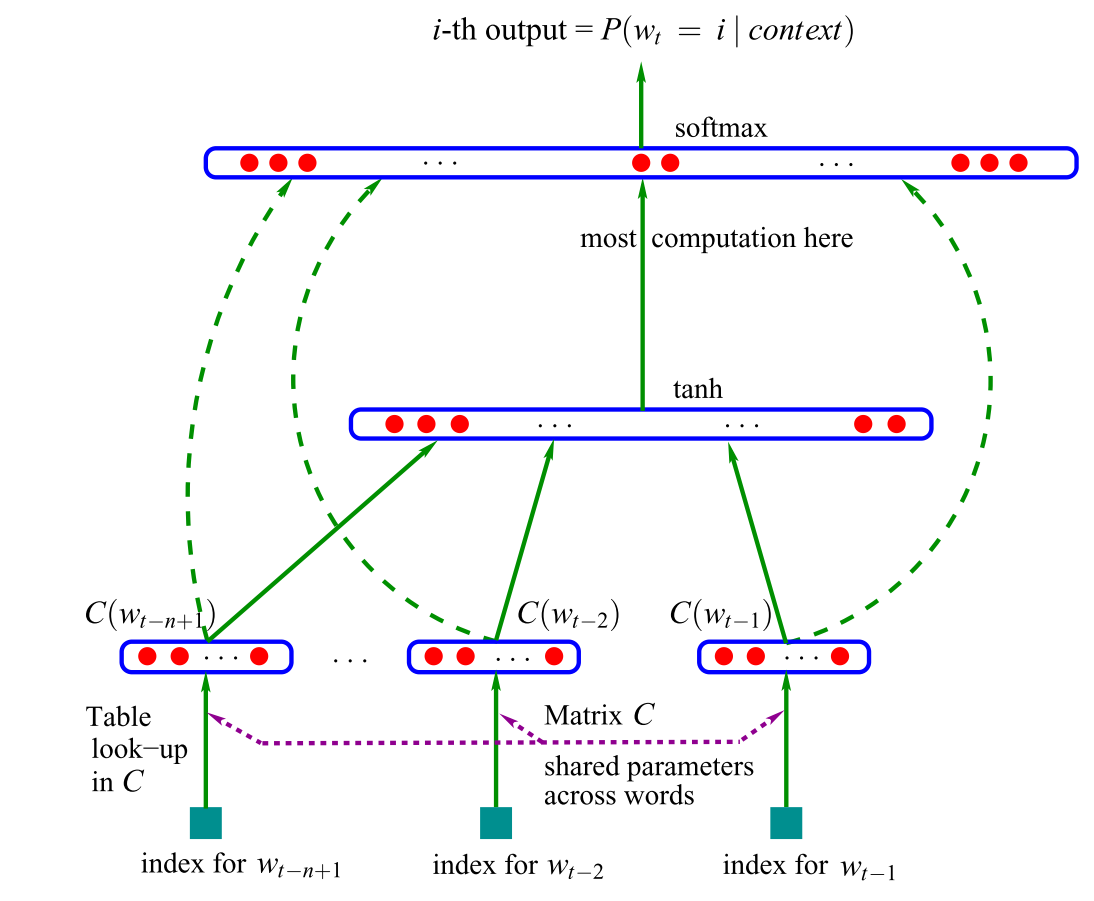
\includegraphics[width=0.5\textwidth]{figures/lm_bengio_2003.png}
 \end{figure}
\let\thefootnote\footnote{\href{https://papers.nips.cc/paper/1839-a-neural-probabilistic-language-model.pdf}{\color[rgb]{0.5,0.5,0.5} [Bengio et al., NIPS ’01]}}
\end{frame}


\begin{frame}[c]{2013 -- Word2vec}
\begin{itemize}
	\setbeamertemplate{itemize items}[square]
	\item Word2vec -- эффективное обучение векторных представлений слов. 
	\item Word2vec предложен в двух вариантах: skip-gram и CBOW.
\end{itemize}
\begin{figure}
	\centering
	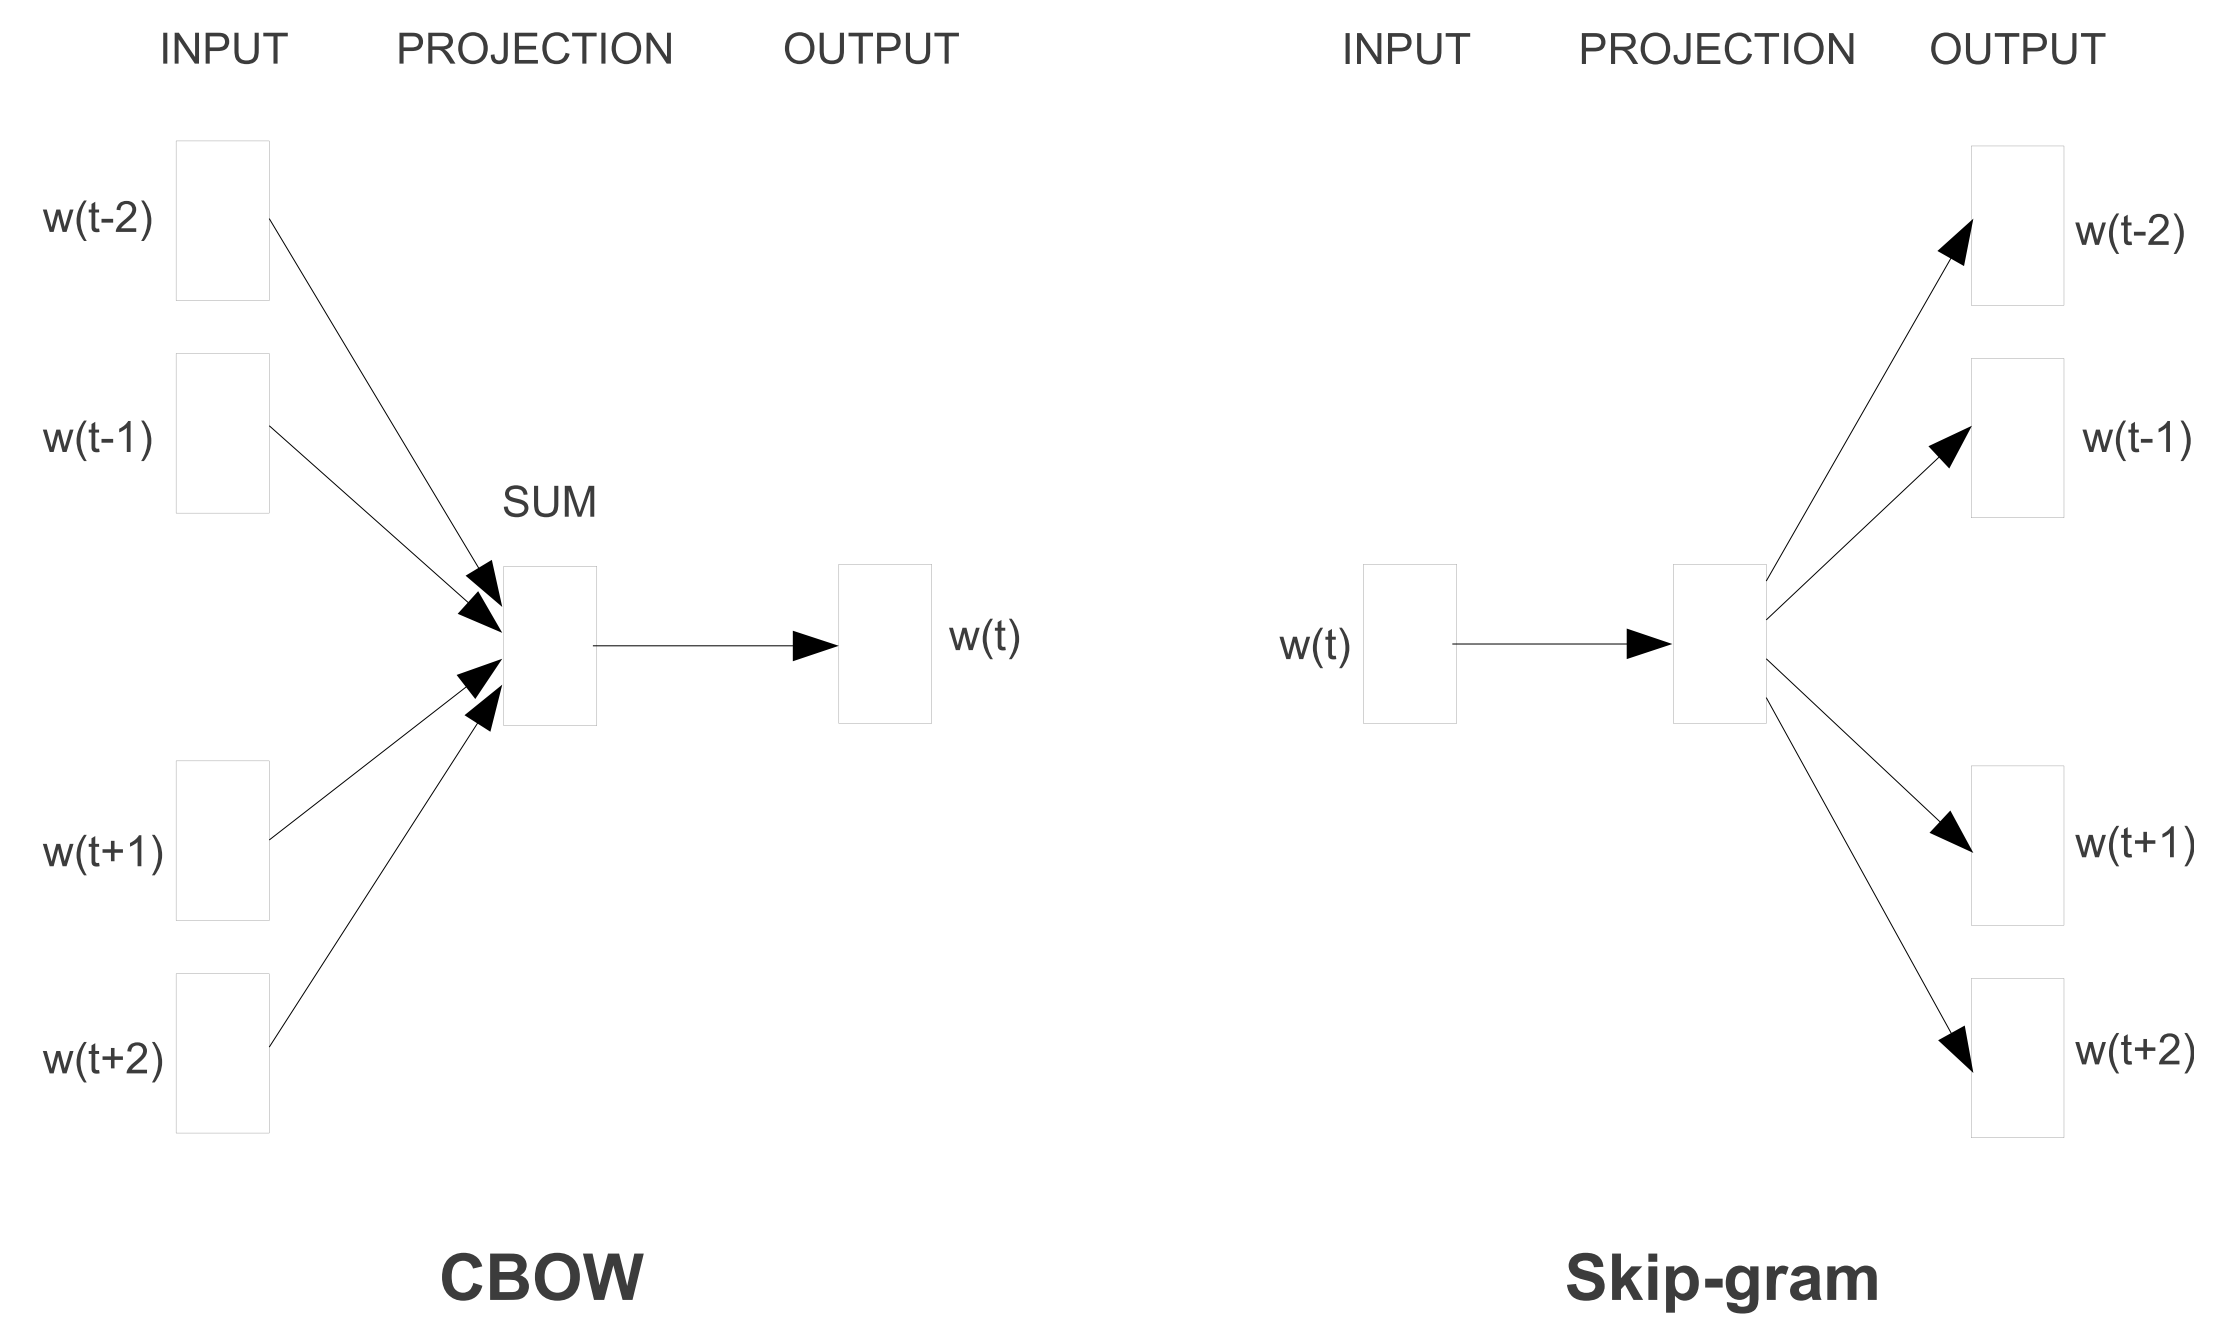
\includegraphics[width=0.8\textwidth]{figures/cbow_skipgram_mikolov_2013.png}
\end{figure}
\let\thefootnote\footnote{\href{http://arxiv.org/abs/1301.3781}{\color[rgb]{0.5,0.5,0.5} [Mikolov et al., ICLR ’13; Mikolov et al., NIPS ’13]}}
\end{frame}

\begin{frame}[c]{2013 -- Нейронные сети}
\begin{itemize}
	\setbeamertemplate{itemize items}[square]
	\item Основная проблема для нейронных сетей -- работа с динамическими входными последовательностями. 
	\item Основные типы:
	\begin{itemize}
		\setbeamertemplate{itemize items}[circle]
		\item Рекуррентные нейронные сети. 
		\item Сверточные нейронные сети.	
	\end{itemize}
\end{itemize}

\end{frame}


\begin{frame}[c]{2013 -- Рекуррентные нейронные сети}
\begin{itemize}
	\setbeamertemplate{itemize items}[square]
	\item Обычный RNN не используются, поскольку градиенты исчезают или взрываются для длинных входов.
	\item Решение: LSTM.
\end{itemize}
\begin{figure}
	\centering
	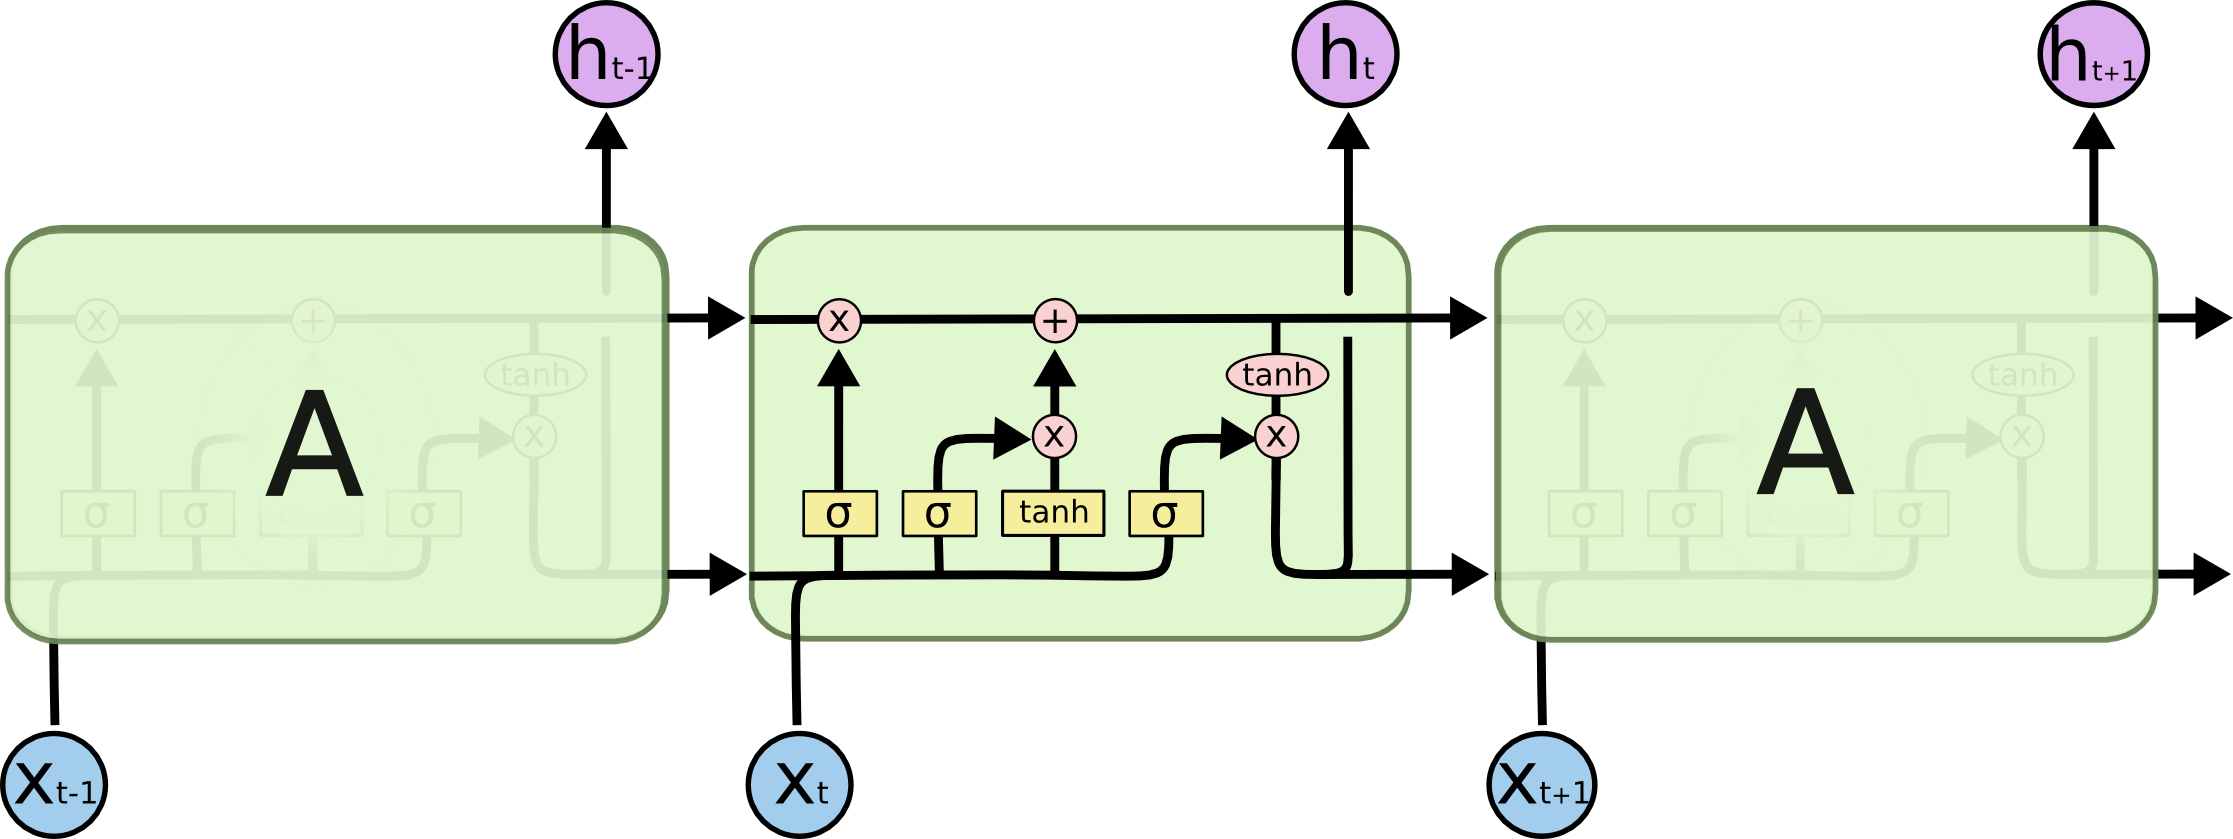
\includegraphics[width=1.0\textwidth]{figures/lstm_colah_2015.png}
\end{figure}
\let\thefootnote\footnote{\href{http://colah.github.io/posts/2015-08-Understanding-LSTMs}{\color[rgb]{0.5,0.5,0.5} [Olah, ’15]}}
\end{frame}

\begin{frame}[c]{2014 -- Сверточные нейронные сети}
\begin{itemize}
	\setbeamertemplate{itemize items}[square]
	\item Одномерная свертка, которая ходит только по ширине.
	\item Max-over-time pooling: max-pooling, примененный ко всей последовательности сразу.
	\item Легко распараллеливается по сравнению с RNN.
	\item Проблема: CNN могут работать только со входом фиксированного размера.
\end{itemize}
\begin{figure}
	\centering
	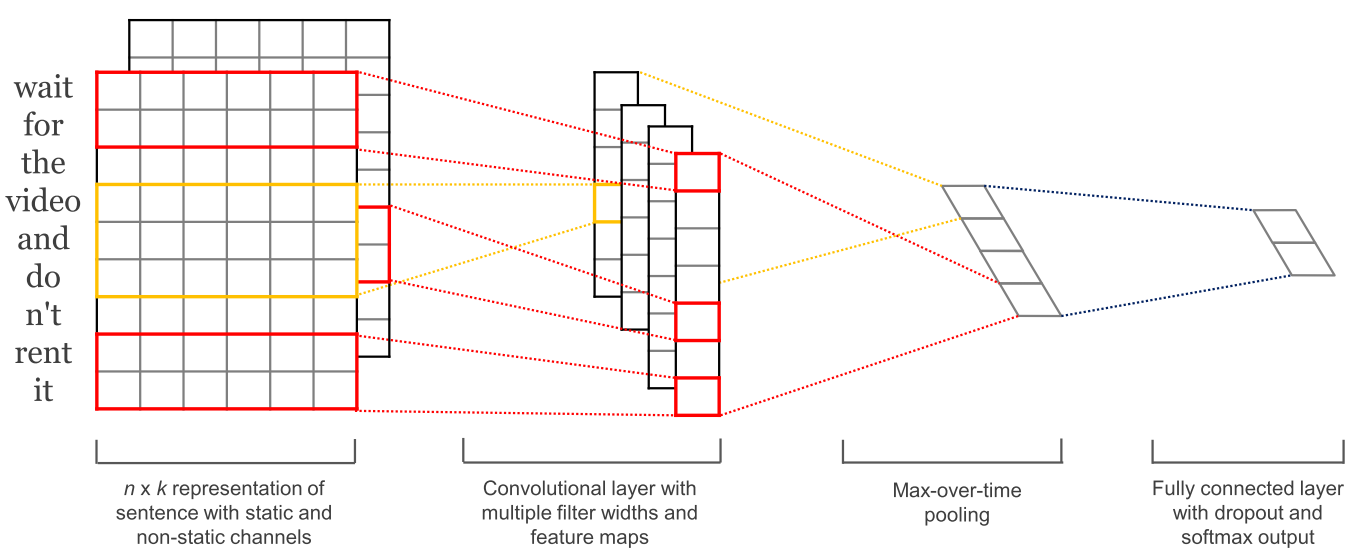
\includegraphics[width=0.8\textwidth]{figures/kim_emnlp2014.png}
\end{figure}
\let\thefootnote\footnote{\href{http://arxiv.org/abs/1408.5882}{\color[rgb]{0.5,0.5,0.5} [Kim, EMNLP ’14]}}
\end{frame}

\begin{frame}[c]{2014 -- seq2seq}
\begin{itemize}
	\setbeamertemplate{itemize items}[square]
	\item Кодировщик обрабатывает вход слово за словом и сжимает его в векторное представление; затем декодировщик предсказывает выход слово за словом на основе состояния кодировщика.
	\item Основное приложение: машинный перевод.
\end{itemize}
\begin{figure}
	\centering
	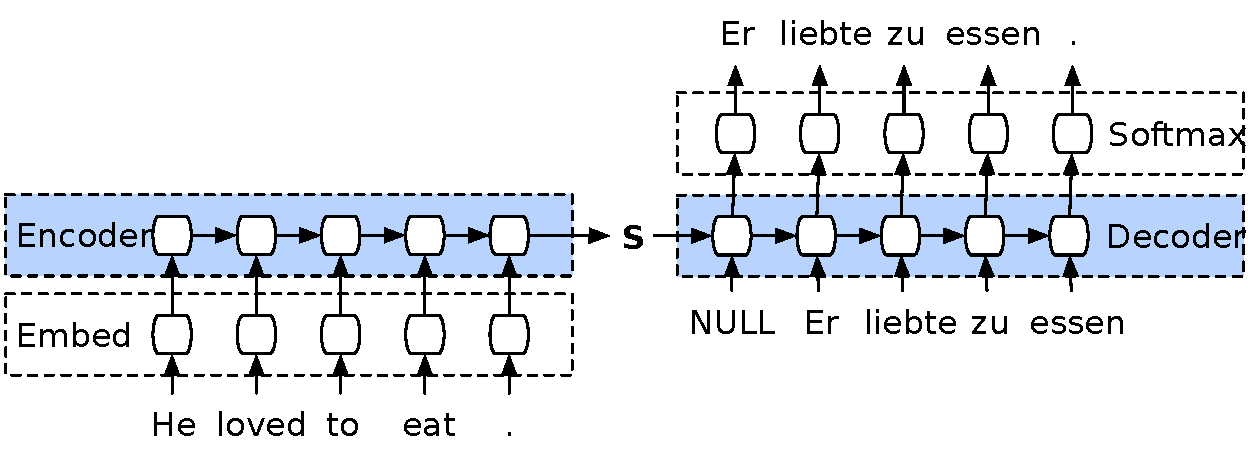
\includegraphics[width=0.9\textwidth]{figures/qseq2seq.pdf}
\end{figure}
\let\thefootnote\footnote{\href{https://arxiv.org/abs/1409.3215}{\color[rgb]{0.5,0.5,0.5} [Sutskever et al., NIPS ’14]}}
\end{frame}

\begin{frame}[c]{2014 -- seq2seq}
\begin{itemize}
	\setbeamertemplate{itemize items}[square]
	\item Для сохранения контекста слова как слева, так и справа используется двунаправленный LSTM.
	\item Проблема: всё предложение целиком сворачивается в вектор фиксированной размерности.
\end{itemize}
\begin{figure}
	\centering
	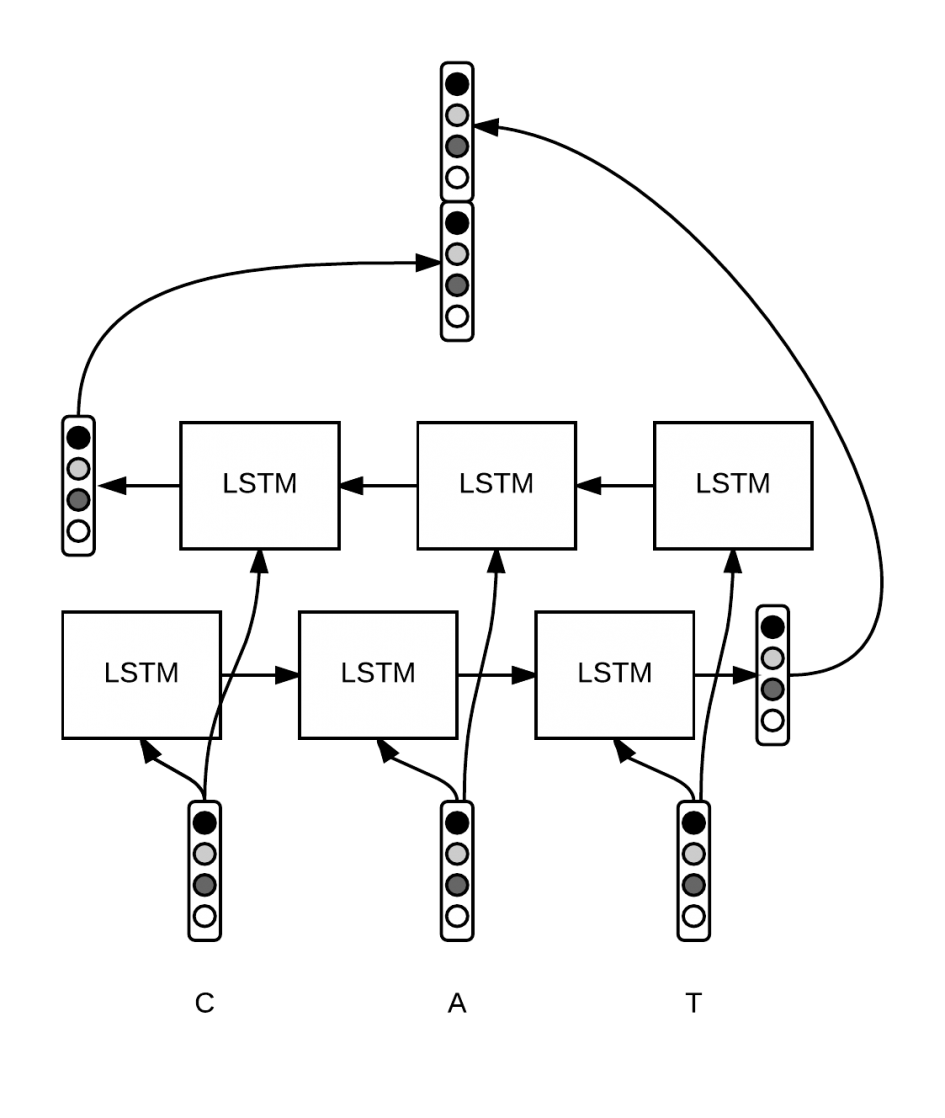
\includegraphics[width=0.4\textwidth]{figures/bilstm.png}
\end{figure}
\end{frame}

\begin{frame}[c]{2015 -- Механизм внимания}
\begin{itemize}
	\setbeamertemplate{itemize items}[square]
	\item Вместо того, чтобы создавать один вектор контекста из последнего скрытого состояния кодировщика, будем использовать взвешенную комбинацию всех входных состояний.
\end{itemize}
\begin{figure}
	\centering
	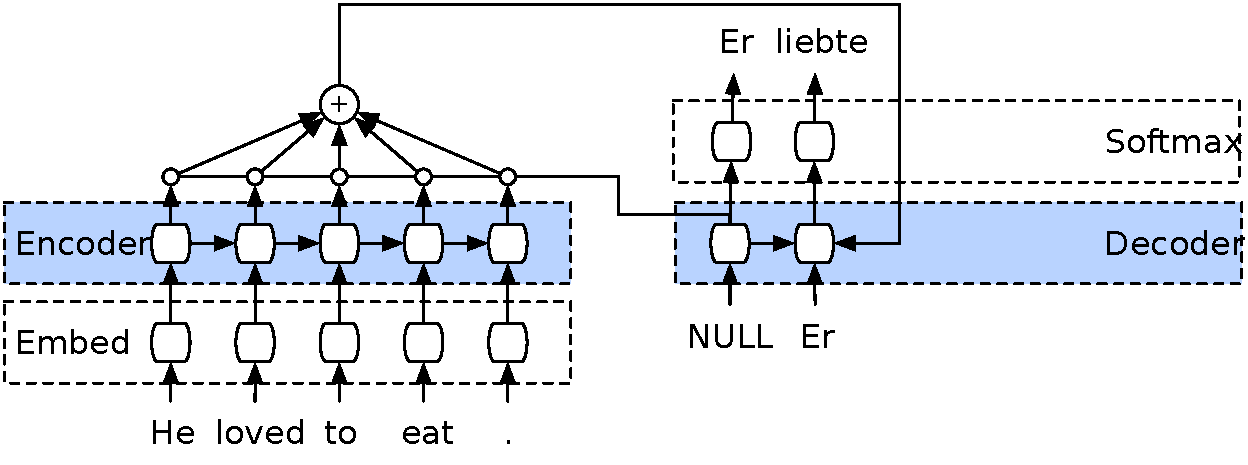
\includegraphics[width=0.9\textwidth]{figures/qseq2seq_a.pdf}
\end{figure}
\let\thefootnote\footnote{\href{http://arxiv.org/abs/1409.0473}{\color[rgb]{0.5,0.5,0.5} [Bahdanau et al., ICLR ’15]}}
\end{frame}

\begin{frame}[c]{2015 -- Механизм внимания}

\begin{columns}
	\begin{column}{0.6\textwidth}
		\begin{itemize}
			\setbeamertemplate{itemize items}[square]
			\item Пусть входная последовательность $x=[x_1,x_2,\cdots,x_T]$, а выходная $y=[y_1,y_2,\cdots,y_M]$.
			\item $h_i = \left[\overrightarrow{h_i}, \overleftarrow{h_i}\right].$
			\item Вектор контекста для выхода $y_t$: $c_t = \sum_{i=1}^{T}\alpha_{ti}h_i$.
			\item Насколько хорошо выровнены $y_t$ и $x_i$: $\alpha_{ti} = \frac{score\left(s_{t-1}, h_i\right)}{\sum_{j=1}^{T}score\left(s_{t-1}, h_j\right)}$.
			\item $score\left(s_{t-1}, h_i\right) = v_a^T \tanh(W_a\left[s_t, h_i\right])$.
		\end{itemize}
	\end{column}
	\begin{column}{0.4\textwidth}
		\begin{figure}
			\centering
			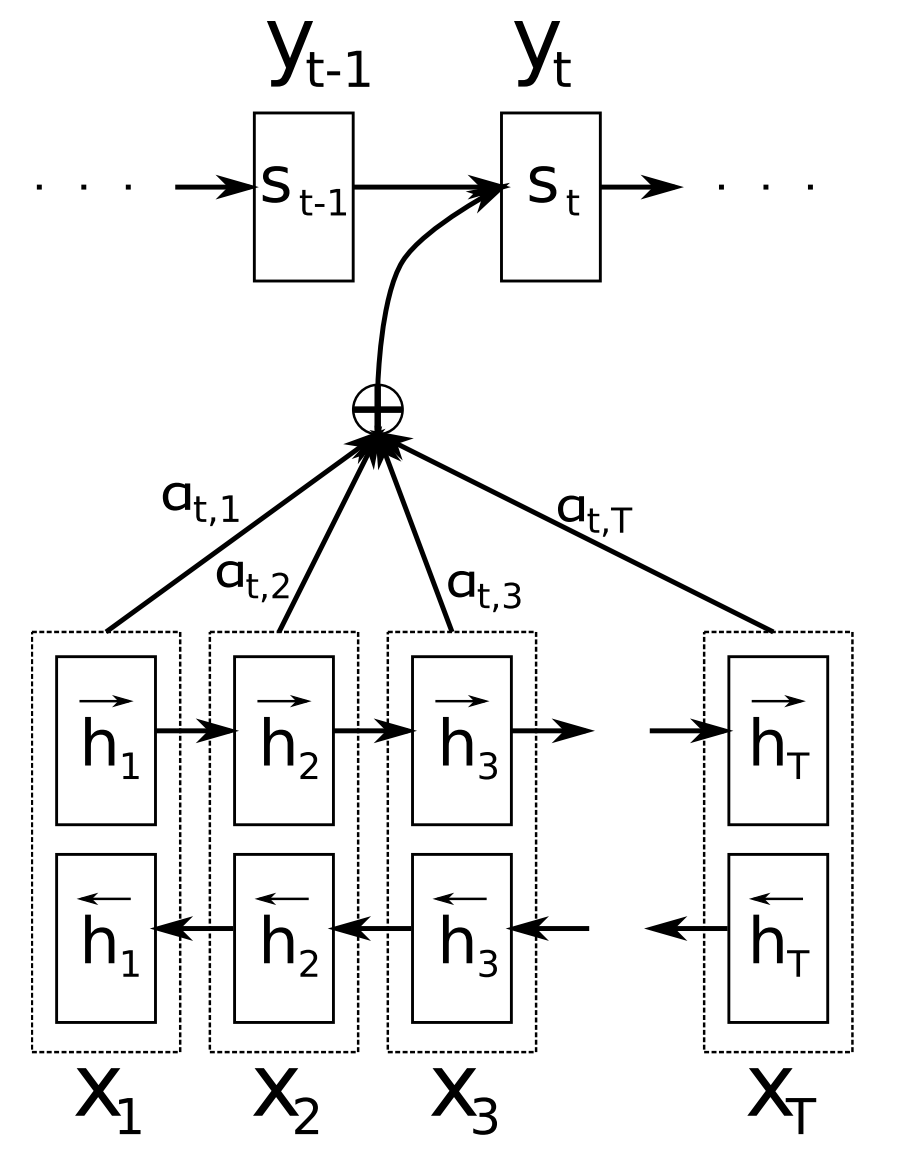
\includegraphics[width=1.0\textwidth]{figures/attention_bahdanau_iclr2015.png}
		\end{figure}
	\end{column}
\end{columns}
\let\thefootnote\footnote{\href{http://arxiv.org/abs/1409.0473}{\color[rgb]{0.5,0.5,0.5} [Bahdanau et al., ICLR ’15]}}
\end{frame}